\documentclass[conference,a4paper]{IEEEtran}
\IEEEoverridecommandlockouts
\usepackage{fontspec}
\usepackage{polyglossia}
\setdefaultlanguage{russian}
\setotherlanguage{english}
\setmainfont{Times New Roman}[Ligatures=TeX]
\newfontfamily\cyrillicfont{Times New Roman}[Ligatures=TeX]
\setsansfont{PT Sans}
\newfontfamily\cyrillicfontsf{PT Sans}
\setmonofont{PT Mono}[Scale=0.9]
\newfontfamily\cyrillicfonttt{PT Mono}[Scale=0.9]
\usepackage{amsmath,amssymb,amsthm}
\usepackage{graphicx}
\usepackage{booktabs}
\usepackage[hidelinks]{hyperref}
\graphicspath{{../results/figures/}}
\sloppy
\emergencystretch=2em

\newtheorem{proposition}{Утверждение}
\theoremstyle{definition}
\newtheorem{definition}{Определение}
\newtheorem{assumption}{Допущение}

\begin{document}

\title{Конформная калибровка открытословарных семантических карт при ошибках метки и позы%
\thanks{Код, данные и подробный отчёт: \url{https://github.com/byoverr/label-pose-conformal-nav}.}}

\author{\IEEEauthorblockN{Сергей Щетинкин}
\IEEEauthorblockA{Университет ИТМО, Санкт-Петербург}}

\maketitle

\begin{abstract}
Робот, который объезжает «растение» по открытословарной семантической карте, получает две ошибки сразу: детектор
пропускает, обрезает или путает объекты, а дрейфующая оценка позы рисует их не там. Гарантии без предположений о
распределении ошибок для планирования по картам восприятия обычно калибруют ошибку восприятия при известной позе. Мы
калибруем одну величину на сцену --- \emph{расстояние промаха}: насколько истинные объекты класса выходят за его область
на карте, построенной по оценённым позам, в системе координат планировщика. Её конформный квантиль даёт запас, который
сертифицирует любой путь, каким бы планировщиком он ни был построен, и отказывается от гарантии, когда она была бы
бесполезной. На 21 сцене OSMa-Bench запасы, откалиброванные только по меткам или только по позе, теряют покрытие под
действием другой ошибки, а сумма двух запасов переплачивает до четверти. Калибровка множеств меток вырождается в запрет
всех занятых клеток. Цену гарантии задаёт наихудшая калибровочная сцена: один пропущенный объект заставляет свой класс
отказываться в 24--63\,\% разбиений. Объединение трёх детекторов снимает отказы, а проверка находок CLIP возвращает их:
гарантия платит за полноту, а не за точность. Если калибровать не карту, а ожидаемую долю опасных миссий, успешных миссий
почти столько же, сколько без калибровки, при 0,6\,\% опасных вместо 7--8\,\%. С реальной одометрией полезной гарантии
нет; SLAM с замыканиями втрое снижает медианную ошибку позы, но запас задают сцены, где замыканий не нашлось.
\end{abstract}

\section{Введение}

Открытословарные семантические карты~\cite{conceptgraphs} позволяют давать роботу задания словами: «не подъезжай к
велосипеду». Карта собирается из двух ненадёжных источников. Метки даёт детектор открытого словаря, и он пропускает
объекты, захватывает их не целиком, путает классы. Положение объектов задаёт оценка позы робота, и она дрейфует.
Планировщик обычно принимает карту за истину и держит фиксированный зазор до запретных объектов.

Насколько это опасно, обычно не измеряют. Бенчмарк OSMa-Bench~\cite{osmabench} показывает, что качество открытословарных
карт сильно падает при смене освещения, но проверяет сегментацию и ответы по графу сцены, а не движение робота; обзор
графов сцены~\cite{survey3dsg} называет связь ошибок карты с поведением робота открытой проблемой. Конформное
предсказание~\cite{gentle} даёт планировщику гарантию без предположений о распределении ошибок, но известные работы
калибруют либо метки~\cite{sundarsingh}, либо раздувание карты занятости~\cite{pwc} и считают позу робота известной, а
отдельно откалиброванные модули не обязаны давать откалиброванную систему~\cite{baral}.

Мы спрашиваем, какую гарантию получает планировщик, когда ошибка метки и ошибка позы действуют вместе, и сколько она
стоит. Вклад работы:
\begin{itemize}
  \item \emph{расстояние промаха} --- поклассовый вариант меры раздувания~\cite{pwc}, измеренный в системе координат
  планировщика на карте по оценённым позам; его конформный квантиль покрывает обе ошибки для любого планировщика;
  \item анализ совместной и раздельной калибровки: сумма двух отдельных запасов гарантирует лишь $1 - 2\alpha$, и то при
  условии, которое из геометрии не следует;
  \item эксперимент на 21 сцене OSMa-Bench с синтетическим дрейфом, реальной одометрией и SLAM, где кроме покрытия
  измерена цена гарантии: запас, доля отказов и доля решённых задач;
  \item проверка того, что снижает цену: ансамбль и каскад детекторов, гарантия на долю опасных миссий вместо гарантии на
  карту, исполнение пути при продолжающемся дрейфе.
\end{itemize}

\section{Связанные работы}

\textbf{Открытословарные карты.} ConceptGraphs~\cite{conceptgraphs} объединяет маски между кадрами в граф объектов с
признаками CLIP. OSMa-Bench~\cite{osmabench} и OSMa-Bench++~\cite{osmabenchpp} оценивают такие карты по сегментации и
вопросам к графу сцены, без задачи движения. Наивное байесовское слияние делает карту переуверенной~\cite{overconf},
поэтому мы сливаем наблюдения усреднением.

\textbf{Конформные гарантии для планирования.} В планирование конформное предсказание пришло через прогноз движения
других агентов~\cite{lindemann}. Yang и др.~\cite{yang2023} калибруют ошибку оценки состояния, но без карты и семантики;
Shin и др.~\cite{shin2026} калибруют поле расстояний до препятствий и называют учёт ошибок восприятия и оценки состояния
будущей работой; Learnable CP~\cite{learnablecp} учит контекстную меру для зазора планировщика. Ближе всего к нам
Sundarsingh и др.~\cite{sundarsingh}: они калибруют множества меток клеток семантической сетки и при известной позе,
пяти классах и открытых площадках $70\times25$~м сообщают 98,36\,\% успешных миссий при цели 95\,\%. Perceive With
Confidence~\cite{pwc} калибрует минимальное раздувание карты занятости, при котором она накрывает все препятствия; наш
промах --- поклассовый вариант этой меры.

\textbf{Композиция и ошибка позы.} Два модуля, откалиброванные на 95\,\% и объединённые как независимые, дают от 99,98
до 86,46\,\% в зависимости от корреляции ошибок~\cite{baral}; распределение риска между модулями через неравенство
Буля~\cite{calafiore2026} требует больше данных. Ошибка позы в семантической памяти плохо откалибрована: номинальный
95\,\%-эллипсоид положения объекта из графа поз накрывает лишь 33\,\% повторных обнаружений~\cite{pposemem}. По
цитированиям ближайших работ и поиску (октябрь 2026~г.) мы не нашли работы, которая совместно калибрует ошибку метки
открытого словаря и ошибку позы с планировщиком в контуре; поиск не исчерпывающий.

\section{Постановка задачи}\label{sec:problem}

Сцена $\Omega$ --- случайный элемент неизвестного распределения $\mathcal D$. Объект $e$ запретного класса
$k_e \in \mathcal K$ имеет след на полу $F_e \subset \mathbb R^2$, и $F_k = \bigcup_{e:\,k_e = k} F_e$. Робот проходит
позы $T_1, \dots, T_Q \in SE(2)$ и в момент $Q$ получает задание. Оценщик выдаёт $\hat T_t = E_t T_t$ с накопленной
плоской ошибкой $E_t$. По наблюдениям и \emph{оценённым} позам строится сетка с шагом $\Delta$; клетка $j$ хранит долю
$p_j(k)$ своих наблюдений, поддерживающих класс $k$. Область класса при пороге $\lambda$ ---
\begin{equation}
  A_\lambda(k) = \{\, c_j : \text{клетка } j \text{ занята},\ p_j(k) \ge \lambda \,\}.
\end{equation}
Робот считает свою позу равной $\hat T_Q$, поэтому в системе планировщика истинный след равен $\hat F_k = E_Q F_k$, а
точка, увиденная в момент $t$, сдвинута относительно него на $E_t E_Q^{-1}$: вредны только относительные ошибки. Путь
$\gamma$ безопасен по классу $k$, если все его точки дальше $d = 0{,}5$~м от $\hat F_k$.

\begin{assumption}[исполнение]\label{as:exec}
Робот проходит путь в системе планировщика, и ошибка позы за время исполнения не меняется.
\end{assumption}

Дано $n$ калибровочных сцен с известной истиной. Нужен запас $\hat r_k \in [0, \infty]$ для каждого класса, возможно
меньший, такой что для новой сцены
\begin{equation}
  \mathbb P\Bigl(\begin{array}{l}\text{любой путь с } \operatorname{dist}(\gamma, A_\lambda(k)) > d + \hat r_k\\
  \text{безопасен по классу } k\end{array}\Bigr) \ge 1 - \alpha.
  \label{eq:goal}
\end{equation}
Значение $\hat r_k = \infty$ (\emph{отказ}) выполняет~\eqref{eq:goal} тривиально.

\begin{assumption}[обменяемость]\label{as:exch}
Пары $(\Omega_i, \xi_i)$ из сцены и реализации ошибок восприятия и позы, $i = 1, \dots, n+1$, обменяемы, а детектор,
карта, $\lambda$ и $R_{\max}$ зафиксированы до калибровки.
\end{assumption}

\section{Метод}\label{sec:method}

\begin{definition}[расстояние промаха]
Для сцены и класса $k$
\begin{equation}
  s_k = \min\bigl\{R_{\max},\ h(\hat F_k, A_\lambda(k))\bigr\},
  \label{eq:miss}
\end{equation}
$h(X, Y) = \max_{x\in X} \min_{y\in Y} \|x - y\|$,
где $\hat F_k$ --- центры клеток истинных объектов в системе планировщика (включая клетки за краем карты), а $h$ ---
направленное расстояние Хаусдорфа; $s_k = 0$, если объектов класса нет, и $R_{\max}$, если область пуста.
\end{definition}

Пропущенный объект даёт большой промах, обрезанный --- длину недорисованной части, сдвиг карты --- порядка сдвига.
Промах считается один на сцену: клетки и кадры одной сцены зависимы и не являются обменяемыми примерами.

\textbf{Калибровка.} Пусть $s^{(1)} \le \dots \le s^{(n)}$ --- упорядоченные калибровочные промахи класса и
$m = \lceil (n+1)(1-\alpha) \rceil$. Запас $\hat r_k = s^{(m)}$, если $m \le n$ и $s^{(m)} < R_{\max}$, иначе отказ.
При $n = 13$ и $\alpha = 0{,}1$ запас равен наибольшему промаху.

\begin{proposition}\label{prop:valid}
При допущениях~\ref{as:exec} и~\ref{as:exch}
$\mathbb P\bigl(\hat r_k = \infty \text{ или } s_k(\Omega_{n+1}) \le \hat r_k\bigr) \ge 1 - \alpha$, и запас выполняет
\eqref{eq:goal} для путей по центрам клеток.
\end{proposition}
\begin{proof}
По обменяемости ранг нового промаха среди $n + 1$ равномерен, поэтому
$\mathbb P(s_k \le s^{(m)}) \ge m/(n+1)$~\cite{gentle}. Если $s_k \le \hat r_k$, то для любой $y \in \hat F_k$ есть
$a \in A_\lambda(k)$ с $\|y - a\| \le \hat r_k$, и для точки пути $x$ с $\operatorname{dist}(x, A_\lambda(k)) > d + \hat r_k$
по неравенству треугольника $\|x - y\| > d$.
\end{proof}

Гарантия не зависит от планировщика: от него зависит лишь, найдётся ли путь в суженном пространстве. Для непрерывного
движения она теряет не больше $\sqrt 2\,\Delta \approx 7$~см; для нескольких классов по неравенству Буля даёт
$1 - |\mathcal K_m|\,\alpha$.

\textbf{Сравниваемые калибровки.} \emph{Без калибровки}: область $A_{\lambda_0}(k)$, запас 0. \emph{Только метки}:
промах карты детектора при точных позах. \emph{Только поза}: промах карты с эталонными метками и дрейфом. \emph{Сумма}
двух этих запасов. \emph{Совместный} (наш): промах карты детектора с дрейфом. Все пять используют порог
$\lambda_0 = 0{,}05$, выбранный на отдельной сцене. \emph{Только геометрия}: областью класса считаются все занятые клетки
--- аналог~\cite{pwc} без семантики; он же служит запасным сертификатом при отказе класса. \emph{Множества
меток}~\cite{sundarsingh}: мера сцены --- худшее $1 - p_j(k)$ по клеткам истинного следа, запретны клетки с
$p_j(k) \ge 1 - \hat\eta$, запаса в метрах нет.

\begin{proposition}\label{prop:sep}
Если $s_k \le s^{\mathrm{lab}}_k + s^{\mathrm{pose}}_k$ для новой сцены, то
$\mathbb P(s_k \le \hat r^{\mathrm{lab}}_k + \hat r^{\mathrm{pose}}_k) \ge 1 - 2\alpha$.
\end{proposition}

Это следует из неравенства Буля. Условие из геометрии не следует: «только поза» измеряет промах эталонной карты, а не
сдвиг предсказанной области, и на наших данных оно нарушается в 2--12\,\% реализаций. Совместный запас от неизвестной
зависимости двух ошибок не зависит.

\textbf{Миссии.} Робот радиуса 0,2~м ищет путь алгоритмом Дейкстры на 8-связной сетке; запретная зона класса ---
клетки ближе $d + \hat r_k$ к его области. Путь \emph{опасен}, если проходит ближе $d$ к истинному запретному объекту;
миссия \emph{успешна}, если путь найден, не опасен и не задевает препятствий. Тот же планировщик на истинной карте даёт
оракул. Гипотезы: запас «только метки» теряет покрытие, когда дрейф сравним с ошибкой меток (H1); «только поза» --- пока
дрейф меньше ошибки меток (H2); совместный запас не больше суммы (H3); mIoU карты слабо связана с безопасностью (H4).
Покрытие совместного запаса не гипотеза: оно следует из утверждения~\ref{prop:valid}.

\section{Экспериментальная установка}

\textbf{Данные и восприятие.} 22 сцены ReplicaCAD~\cite{habitat2} из OSMa-Bench~\cite{osmabench}: RGB-D, эталонная
семантика и позы, каждый 8-й кадр. Все решения о методе приняты на сцене \texttt{apt\_0}, которая не входит ни в
калибровку, ни в тест. Детектор YOLO-World v2-s~\cite{yoloworld} с 98 текстовыми запросами; внутри рамки остаются
пиксели не дальше 0,25~м от медианной глубины. Сетка 5~см. Запретные классы --- растение, велосипед и тумба под ТВ.

\textbf{Ошибка позы.} Синтетический дрейф повторяет каждое относительное движение траектории с плоским шумом,
пропорциональным пройденному пути и углу поворота. Пять уровней заданы по опубликованным ошибкам реальных систем; на
тестовых сценах медианная ATE равна 0,4~см (L1), 2~см (L2), 7~см (L3), 45~см (L4) и 2,7~м (L5), по 10 реализаций.
Реальная ошибка --- RGB-D-одометрия Open3D~\cite{open3d,steinbrucker} без замыканий циклов и наш SLAM с замыканиями.

\textbf{Протокол.} $\alpha = 0{,}1$, $R_{\max} = 3$~м. 21 сцена 200 раз делится на 13 калибровочных и 8 тестовых.
Покрытие --- доля тестовых реализаций, где промах не больше запаса; отказ засчитывается как пустая гарантия, и отдельно
приводится доля отказов. Разбиения берутся из одних и тех же сцен, поэтому покрытие совместного запаса выполняется по
построению; содержательны запас, отказы и поведение вариантов без гарантии. \emph{Трудные} задачи отобраны так, что
кратчайший путь по одной геометрии проходит ближе 0,5~м к растению или велосипеду (233 задачи в 15 сценах);
\emph{случайные} --- по 20 на сцену. Запасы для сцены калибруются по остальным 20 сценам. Семейство задач и пара
запретных классов выбраны после первых прогонов.

\section{Результаты}

\begin{table*}[t]
\centering
\caption{Покрытие и медианный запас $\hat r$ по 200 разбиениям 13/8, $1 - \alpha = 0{,}9$; медианная ATE L2 --- 2~см,
L3 --- 7~см, L4 --- 45~см. Отказ засчитан как покрытие; $^\dagger$ --- вариант отказывается в половине разбиений или
чаще, приведён запас остальных. Запас «только геометрия» отсчитывается от всех занятых клеток.}
\label{tab:coverage}
\footnotesize
\begin{tabular}{llcccccccc}
\toprule
Класс & Калибровка & \multicolumn{2}{c}{L0} & \multicolumn{2}{c}{L2} & \multicolumn{2}{c}{L3} & \multicolumn{2}{c}{L4} \\
 & & покр. & $\hat r$, м & покр. & $\hat r$, м & покр. & $\hat r$, м & покр. & $\hat r$, м \\
\midrule
велосипед & без калибровки & 0{,}00 & 0 & 0{,}00 & 0 & 0{,}01 & 0 & 0{,}01 & 0 \\
 & метки клеток & 1{,}00 & 0 & 0{,}73 & 0 & 0{,}34 & 0 & 0{,}17 & 0 \\
 & только метки & 0{,}93 & 0{,}75 & 0{,}94 & 0{,}75 & 0{,}93 & 0{,}75 & 0{,}76 & 0{,}75 \\
 & только поза & 0{,}00 & 0{,}00 & 0{,}03 & 0{,}07 & 0{,}22 & 0{,}18 & 0{,}82 & 0{,}90 \\
 & раздельно & 0{,}93 & 0{,}75 & 0{,}98 & 0{,}82 & 0{,}99 & 0{,}90 & 0{,}97 & 1{,}61 \\
 & \textbf{совместно} & 0{,}93 & 0{,}75 & 0{,}94 & 0{,}75 & 0{,}94 & 0{,}75 & 0{,}93 & 1{,}18 \\
\midrule
растение & без калибровки & 0{,}00 & 0 & 0{,}00 & 0 & 0{,}00 & 0 & 0{,}00 & 0 \\
 & метки клеток & 1{,}00 & 0 & 0{,}41 & 0 & 0{,}10 & 0 & 0{,}03 & 0 \\
 & только метки & 0{,}93 & отк.\,0{,}63 & 0{,}96 & отк.\,0{,}64 & 0{,}94 & отк.\,0{,}64 & 0{,}86 & отк.\,0{,}64 \\
 & только поза & 0{,}00 & 0{,}00 & 0{,}00 & 0{,}11 & 0{,}13 & 0{,}25 & 0{,}86 & 1{,}39 \\
 & раздельно & 0{,}93 & отк.\,0{,}63 & 0{,}98 & отк.\,0{,}64 & 0{,}96 & отк.\,0{,}64 & 0{,}95 & отк.\,0{,}64 \\
 & \textbf{совместно} & 0{,}93 & отк.\,0{,}63 & 0{,}93 & 0{,}80 & 0{,}94 & отк.\,0{,}55 & 0{,}93 & отк.\,0{,}58 \\
\midrule
тумба под ТВ & без калибровки & 0{,}05 & 0 & 0{,}01 & 0 & 0{,}00 & 0 & 0{,}00 & 0 \\
 & метки клеток & 1{,}00 & 0 & 0{,}77 & 0 & 0{,}61 & 0 & 0{,}30 & 0 \\
 & только метки & 0{,}98 & отк.\,0{,}95 & 0{,}98 & отк.\,0{,}95 & 0{,}98 & отк.\,0{,}95 & 0{,}99 & отк.\,0{,}95 \\
 & только поза & 0{,}05 & 0{,}00 & 0{,}06 & 0{,}07 & 0{,}13 & 0{,}16 & 0{,}47 & 0{,}56 \\
 & раздельно & 0{,}98 & отк.\,0{,}95 & 0{,}98 & отк.\,0{,}95 & 0{,}98 & отк.\,0{,}95 & 1{,}00 & отк.\,0{,}95 \\
 & \textbf{совместно} & 0{,}98 & отк.\,0{,}95 & 0{,}98 & отк.\,0{,}94 & 0{,}97 & отк.\,0{,}93 & 0{,}94 & отк.\,0{,}72 \\
\bottomrule
\end{tabular}

\end{table*}

\subsection{Покрытие при дрейфе позы}

Карта без калибровки почти никогда не содержит истинный след целиком: детектор обрезает края объектов
(табл.~\ref{tab:coverage}). Множества меток дают 1,00 при точной позе лишь потому, что их порог нулевой: во всех 21
сцене у каждого класса есть занятая клетка следа без единого наблюдения этого класса, и запретными становятся все
занятые клетки. Без запаса в метрах уже 2~см дрейфа снижают их покрытие велосипеда до 0,73. Запас «только метки» держится,
пока дрейф меньше ошибки меток, и падает до 0,76 для велосипеда при 45~см (90\,\%-интервал бутстрепа 0,67--0,82, H1);
«только поза» не видит ошибок детектора и до 7~см не выше 0,27 (H2). Сумма переплачивает: при 45~см совместный запас
меньше на 23--25\,\% (1,23 против 1,61~м для велосипеда), при 0,4--7~см --- на 6--25\,\% (H3).

Совместный запас держит 0,92--0,94, как и должен. Важны его цена и отказы. Велосипед сертифицируется на всех уровнях до
L4, запас растёт с 0,75 до 1,23~м. Растение в одной из 21 сцены пропущено целиком, и при 13 калибровочных сценах класс
отказывается всякий раз, когда эта сцена попадает в калибровку: в 24--63\,\% разбиений. Тумбу детектор уверенно путает
со скамейкой, ковром или кроватью в трёх сценах, и она отказывается в 75--95\,\% разбиений.

\subsection{Миссии}

\begin{figure}[t]
\centering
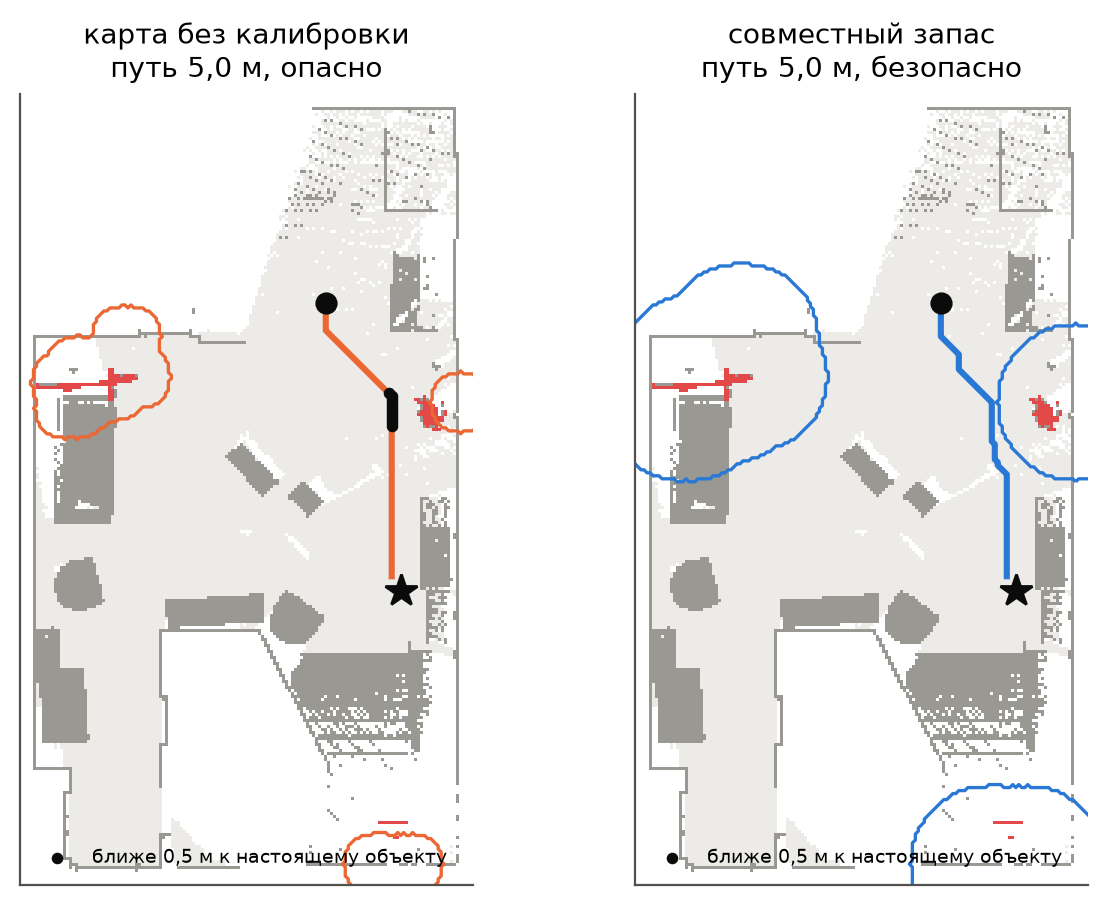
\includegraphics[width=\linewidth]{ru/example_v3_sc0_staging_20_ru.png}
\caption{Трудная задача при дрейфе 2~см в системе планировщика. Без калибровки запретная зона не накрывает обрезанный
край растения, и путь проходит ближе 0,5~м к нему (чёрные точки); совместный запас накрывает объект.}
\label{fig:example}
\end{figure}

\begin{table*}[t]
\centering
\caption{Трудные задачи (растение и велосипед, 233 задачи в 15 сценах, при дрейфе --- 5 реализаций): доля задач с
путём, число опасных путей из найденных, доля успешных миссий.}
\label{tab:missions}
\footnotesize
\begin{tabular}{lccccccccc}
\toprule
Ветка & \multicolumn{3}{c}{L0} & \multicolumn{3}{c}{L2} & \multicolumn{3}{c}{L4} \\
 & путь & наруш. & успех & путь & наруш. & успех & путь & наруш. & успех \\
\midrule
без калибровки & 0{,}99 & 0{,}27 & 0{,}73 & 0{,}97 & 0{,}32 & 0{,}65 & 0{,}26 & 0{,}34 & 0{,}17 \\
покадровая CP меток & 0{,}27 & 0{,}00 & 0{,}27 & 0{,}28 & 0{,}00 & 0{,}28 & 0{,}04 & 0{,}23 & 0{,}03 \\
только метки & 0{,}32 & 0{,}00 & 0{,}32 & 0{,}31 & 0{,}00 & 0{,}31 & 0{,}10 & 0{,}00 & 0{,}10 \\
только поза & 0{,}99 & 0{,}27 & 0{,}73 & 0{,}96 & 0{,}20 & 0{,}77 & 0{,}09 & 0{,}00 & 0{,}09 \\
раздельно (сумма) & 0{,}32 & 0{,}00 & 0{,}32 & 0{,}31 & 0{,}00 & 0{,}31 & 0{,}00 & 0{,}00 & 0{,}00 \\
\textbf{совместно} & 0{,}32 & 0{,}00 & 0{,}32 & 0{,}31 & 0{,}00 & 0{,}31 & 0{,}03 & 0{,}00 & 0{,}03 \\
оракул & 1{,}00 & 0{,}00 & 1{,}00 & 0{,}98 & 0{,}00 & 0{,}98 & 0{,}98 & 0{,}00 & 0{,}98 \\
\bottomrule
\end{tabular}

\end{table*}

На трудных задачах планировщик без калибровки почти всегда находит путь, но 54--58\,\% его путей опасны: он срезает
обрезанный край объекта (рис.~\ref{fig:example}, табл.~\ref{tab:missions}). У совместного запаса опасны 0--2 пути из
74--364, а опасная клетка достижима для какого-нибудь планировщика в 0--3\,\% реализаций против 96--100\,\%. Множества
меток безопасны при точной позе, но при 2 и 7~см опасны 9 и 27\,\% их путей. Цена --- путь находится лишь в 30--32\,\%
нарочно трудных задач против 97--100\,\% на истинной карте: гарантия ограничивает риск, а не повышает успех. Семантика
окупается: запас без неё («только геометрия») решает при дрейфе в 2--6 раз меньше задач. На случайных задачах совместный
запас успешен в 78\,\% миссий при точной позе и в 68\,\% при 7~см без опасных путей; без калибровки --- 93 и 80\,\%, но
7--8\,\% путей опасны. Ранговая корреляция mIoU карты с долей опасных путей по 15 сценам 0,18 (интервал от $-0{,}35$ до
$0{,}68$): связи не видно, но и её отсутствие не доказано (H4).

\subsection{Сравнение с множествами меток}

\begin{table*}[t]
\centering
\caption{Случайные задачи (420 в 21 сцене): доля успешных миссий; $^\ast$ --- есть опасные пути.}
\label{tab:comparison}
\footnotesize
\begin{tabular}{ll|ccc|ccc|cc|c}
\toprule
Условия & Дрейф & \multicolumn{3}{c|}{метки клеток} & \multicolumn{3}{c|}{\textbf{совместно}} & \multicolumn{2}{c|}{без калибровки} & оракул \\
 & & покр. & успех & опасно & покр. & успех & опасно & успех & опасно & успех \\
\midrule
закрытый словарь, 95\,\% & известна & 1{,}00 & 0{,}43 & 0{,}000 & 0{,}94 & 0{,}42 & 0{,}000 & 0{,}96 & 0{,}040 & 1{,}00 \\
 & L2 & 0{,}42 & 0{,}40 & 0{,}000 & 0{,}94 & 0{,}61 & 0{,}000 & 0{,}92 & 0{,}042 & 0{,}97 \\
 & L3 & 0{,}10 & 0{,}32 & 0{,}002 & 0{,}94 & 0{,}50 & 0{,}000 & 0{,}82 & 0{,}049 & 0{,}97 \\
\midrule
открытый словарь, 90\,\% & известна & 1{,}00 & 0{,}43 & 0{,}000 & 0{,}93 & 0{,}78 & 0{,}000 & 0{,}95 & 0{,}043 & 1{,}00 \\
 & L2 & 0{,}41 & 0{,}40 & 0{,}000 & 0{,}93 & 0{,}74 & 0{,}000 & 0{,}91 & 0{,}050 & 0{,}97 \\
 & L3 & 0{,}10 & 0{,}32 & 0{,}002 & 0{,}94 & 0{,}68 & 0{,}000 & 0{,}82 & 0{,}056 & 0{,}97 \\
 & L4 & 0{,}03 & 0{,}09 & 0{,}000 & 0{,}93 & 0{,}17 & 0{,}000 & 0{,}29 & 0{,}021 & 0{,}98 \\
\bottomrule
\end{tabular}

\end{table*}

Успех миссий~\cite{sundarsingh} получен в другой постановке, поэтому мы сравниваем методы на наших сценах по схеме
$2 \times 2$: закрытый словарь из пяти классов или открытый, $1 - \alpha = 0{,}95$ (как у авторов) или 0,9. Множества
меток дают одно и то же во всех четырёх вариантах: порог всегда нулевой, и запрещено всё занятое (43\,\% успешных
миссий). В их условиях (0,95, известная поза) совместный запас с ними совпадает (42\,\%): растение отказывается и
переходит на ту же зону. Разницу при известной позе создаёт уровень риска, а не словарь: при 0,9 совместный запас успешен
в 78\,\% миссий. При дрейфе множества меток пропускают опасные пути, а совместный запас --- нет. Наши абсолютные числа
ниже 98,36\,\% у~\cite{sundarsingh}, но их метод на наших сценах даёт 43\,\%: разрыв создаёт постановка, а не метод
(табл.~\ref{tab:comparison}). Множество меток может сказать лишь «эта клетка может быть растением»; расстояние говорит
«растение где-то рядом», и это остаётся полезным, когда детектор теряет края объектов.

\subsection{Цена гарантии и что её снижает}

Повышение $\alpha$ с 0,1 до 0,3 почти не добавляет решаемых задач (30 → 31\,\% трудных при 7~см): запас задаёт
наихудшая калибровочная сцена, пока $n < 2/\alpha - 1$. При 19 калибровочных сценах одна сцена с пропущенным растением
перестаёт определять запас, и отказы растения падают с 63 до 0\,\% без дрейфа. Более строгая PAC-форма
гарантии~\cite{vovk} при 20 сценах невозможна. Маски MobileSAM~\cite{mobilesam}, доращивание областей, иерархическая
калибровка~\cite{hcp} и условный запас по длине пути цену почти не меняют.

\begin{table*}[t]
\centering
\caption{Детекторы с одним словарём из 98 классов, их объединение (в клетке --- максимум, среднее или второе по величине
из трёх долей класса) и каскад с проверкой CLIP: медианный запас совместного варианта (м) и доля разбиений с отказом;
доля трудных задач с путём и доля успешных случайных миссий.}
\label{tab:detector}
\footnotesize
\begin{tabular}{l|cc|cc|cc|cc}
\toprule
Детектор & \multicolumn{2}{c|}{растение: $\hat r$ / отказ} & \multicolumn{2}{c|}{велосипед: $\hat r$} & \multicolumn{2}{c|}{трудные: путь} & \multicolumn{2}{c}{случайные: успех} \\
 & L0 & L4 & L0 & L4 & L0 & L3 & L0 & L3 \\
\midrule
YOLO-World v2-s & 0{,}85 / 0{,}63 & 1{,}54 / 0{,}59 & 0{,}75 & 1{,}23 & 0{,}32 & 0{,}30 & 0{,}78 & 0{,}68 \\
YOLO-World v2-x & 0{,}71 / 0{,}00 & 1{,}56 / 0{,}10 & 0{,}80 & 1{,}11 & 0{,}41 & 0{,}23 & 0{,}83 & 0{,}64 \\
\bottomrule
\end{tabular}

\end{table*}

\textbf{Детекторы.} Худший промах растения дают два маленьких горшка в одной сцене. YOLO-World v2-x и
YOLOE~\cite{yoloe} их находят, но у каждого детектора свой целиком пропущенный класс: v2-x теряет тумбу, YOLOE ---
велосипед в двух сценах (табл.~\ref{tab:detector}). Объединение трёх карт по максимуму снимает отказы всех трёх
классов до 45~см (тумба: 0\,\% вместо 74--95\,\%), и путь находится в 60\,\% трудных задач без дрейфа и в 47\,\% при
2~см вместо 32 и 31\,\%; при 7~см --- в 22\,\% вместо 30\,\%, потому что в одной сцене ансамбль наконец видит растение и
закрывает проход. Среднее и согласие двух детекторов хуже. Каскад, в котором находки проверяет CLIP~\cite{clip} по
вырезке рамки, выбрасывает растение и тумбу целиком в трёх сценах, а голосование по кадрам увеличивает промахи уже на
отладочной сцене. Гарантия платит за наихудший промах, поэтому выигрывает полнота: проверка, которая может только убирать
находки, только добавляет промахов. Идея ансамбля возникла после того, как мы увидели пропуски детекторов на этих сценах,
поэтому выигрыш может быть оптимистичным.

\subsection{Гарантия на миссии и исполнение}

\begin{table*}[t]
\centering
\caption{Гарантии разной силы на одних и тех же задачах: доля успешных миссий при точной позе, 2 и 7~см и наибольшая по
уровням доля опасных миссий. Совместный запас и риск пути гарантируют каждый путь, риск планировщика --- ожидаемую долю
опасных миссий в новой сцене; «по исполнению» --- с учётом дрейфа во время движения.}
\label{tab:crc}
\footnotesize
\begin{tabular}{ll|ccc|c|ccc|c}
\toprule
Правило & Уровень & \multicolumn{4}{c|}{случайные задачи} & \multicolumn{4}{c}{трудные задачи} \\
 & & L0 & L2 & L3 & опасн. & L0 & L2 & L3 & опасн. \\
\midrule
без калибровки & --- & 0{,}93 & 0{,}88 & 0{,}80 & 0{,}076 & 0{,}45 & 0{,}41 & 0{,}39 & 0{,}563 \\
совместный запас & $\alpha = 0{,}1$ на класс & 0{,}78 & 0{,}74 & 0{,}68 & 0{,}000 & 0{,}32 & 0{,}31 & 0{,}30 & 0{,}002 \\
риск пути & $a = 0{,}2$ & 0{,}77 & 0{,}70 & 0{,}71 & 0{,}000 & 0{,}29 & 0{,}29 & 0{,}27 & 0{,}002 \\
риск планировщика & $a = 0{,}05$ & 0{,}94 & 0{,}87 & 0{,}80 & 0{,}006 & 0{,}00 & 0{,}00 & 0{,}00 & 0{,}000 \\
риск планировщика & $a = 0{,}1$ & 0{,}95 & 0{,}92 & 0{,}88 & 0{,}051 & 0{,}40 & 0{,}57 & 0{,}36 & 0{,}013 \\
то же, по исполнению & $a = 0{,}1$ & --- & 0{,}92 & 0{,}87 & 0{,}052 & --- & 0{,}56 & 0{,}36 & 0{,}011 \\
риск планировщика, ансамбль & $a = 0{,}05$ & 0{,}91 & 0{,}86 & 0{,}75 & 0{,}027 & 0{,}00 & 0{,}00 & 0{,}00 & 0{,}000 \\
риск планировщика, ансамбль & $a = 0{,}1$ & 0{,}96 & 0{,}92 & 0{,}86 & 0{,}043 & 0{,}41 & 0{,}83 & 0{,}54 & 0{,}022 \\
\bottomrule
\end{tabular}

\end{table*}

Вместо отказа можно сообщать для пути конформную оценку риска: путь с зазором $c$ до области класса опасен, только если
$s_k > c$, поэтому $\rho_k(c) = (1 + \#\{i : s_{i,k} \ge c\})/(n+1)$ --- конформное p-значение даже для пути, выбранного
по тестовой карте. Решаемость та же, что у совместного запаса, но робот получает путь с явным риском.

Совместный запас обещает, что внутри него лежит \emph{каждый} объект класса, в том числе тот, мимо которого не идёт ни
один путь. Роботу важнее доля опасных миссий, и её можно калибровать напрямую контролем конформного риска~\cite{crc} по
запасу планировщика: для запаса $m$ потеря сцены $L_i(m)$ --- доля её опасных миссий, и наименьший $m$ с
$(\sum_i \tilde L_i(m) + 1)/(n+1) \le a$, где $\tilde L_i$ --- монотонная огибающая, даёт $\mathbb E[L_{\text{тест}}] \le a$.
В планировании этот приём уже применяли~\cite{gonzales,eom}, но не к семантическим картам с ошибкой позы. На случайных
задачах при $a = 0{,}05$ успешны 94, 87 и 80\,\% миссий при точной позе, 2 и 7~см --- почти как без калибровки (93, 88,
80\,\%), но опасных не больше 0,6\,\% вместо 7--8\,\% (табл.~\ref{tab:crc}). Гарантия слабее: отдельная сцена может быть
опасной целиком (в худшей --- 13\,\%). Вместе с ансамблем детекторов при $a = 0{,}1$ путь находится в 41, 83 и 54\,\%
трудных задач при не более 2,2\,\% опасных --- лучшее сочетание из проверенных.

Основная гарантия относится к плану (допущение~\ref{as:exec}). Когда робот едет по плану, а оценка позы продолжает
дрейфовать, при 2--7~см отклонение составляет 0,3--0,8\,\% пройденного пути, и пути, сертифицированные по плану,
остаются безопасными (опасных исполнений не больше 0,6\,\%). При 45~см 18\,\% сертифицированных путей задевают
препятствия, а откалиброванный запас на исполнение (около 17~см на метр пути) делает сертификат почти недостижимым:
нужна перелокализация во время движения. Контроль риска с потерей «опасно при исполнении» покрывает и движение: при
$a = 0{,}05$ успешны 87 и 80\,\% случайных миссий при 2 и 7~см.

\subsection{Реальная локализация и другие сцены}

RGB-D-одометрия без замыканий ошибается скачками на поворотах у стен; медианная ATE 78~см. Запас «только метки» молча
теряет покрытие (0,62 для велосипеда), а совместный формально валиден лишь потому, что отказывается в 86\,\% разбиений.
SLAM с замыканиями поверх той же одометрии (граф поз по схеме~\cite{choi2015}, кандидаты по ORB и PnP) снижает медианную
ATE до 24~см, и совместный запас велосипеда 1,59~м сертифицирует без отказов при покрытии 0,92. Но в двух сценах
замыканий не нашлось (2--3~м ошибки), и запас задают они: путь находится лишь в 1\,\% трудных задач. Решает хвост ошибок
локализации, а не медиана. На сценах HM3D~\cite{hm3d} гарантия с ReplicaCAD не переносится (один контрпример из двух
сцен с видимым растением). Сумма отдельных запасов может и недопокрывать (рис.~\ref{fig:composition}): если редкие сбои локализации приходятся
на сцены с хорошими метками, её покрытие опускается до 0,66--0,69 при цели 0,70, а совместный запас держит 0,69--0,74
при любом расположении сбоев.

\begin{figure}[t]
\centering
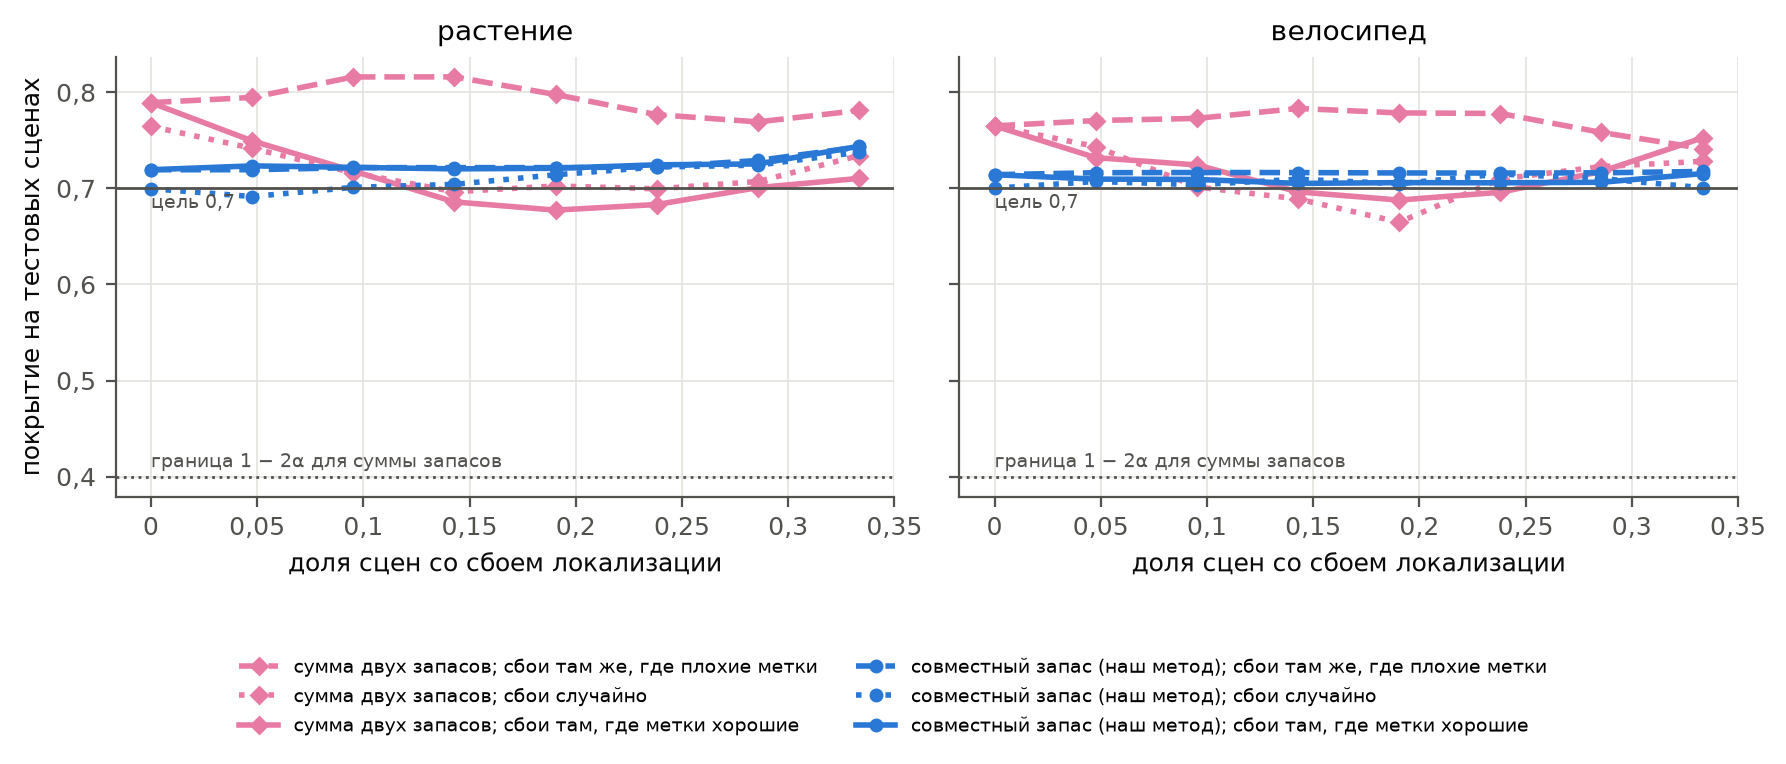
\includegraphics[width=\linewidth]{ru/composition_stress.png}
\caption{Покрытие суммы отдельных запасов и совместного запаса в зависимости от доли сцен со сбоем локализации;
$1 - \alpha = 0{,}7$, пунктир --- граница $1 - 2\alpha$ для суммы.}
\label{fig:composition}
\end{figure}

\section{Обсуждение и ограничения}

Главное узкое место --- уверенный пропуск или подмена класса целого объекта. Пока калибровочных сцен меньше
$2/\alpha - 1$, запас равен наихудшему промаху, и одна такая сцена заставляет класс отказываться. Объединение детекторов
снимает его, гарантия на миссии делает цену приемлемой, но выбор между гарантиями --- вопрос требований: «ни один объект
не выйдет за запас» или «в среднем не больше $a$ опасных миссий». Метрики карты вроде mIoU этого не видят, и в протокол
бенчмарков естественно добавить долю сцен с целиком пропущенным объектом.

Ограничения: одно семейство из 21 симулированной сцены; покрытие на разбиениях одних и тех же сцен выполняется по
построению; основной дрейф синтетический; восприятие --- детектор рамок, а не полный картограф; гарантия поклассовая и
маргинальная; семейство трудных задач и пара запретных классов выбраны после первых прогонов.

\section{Заключение}

Расстояние промаха в системе координат планировщика --- одна калибруемая величина, которая даёт гарантию сразу против
ошибки метки и ошибки позы и честно отказывается, когда гарантия была бы бесполезной. Запасы по одной ошибке теряют
покрытие под действием другой, сумма отдельных запасов переплачивает или недопокрывает, а множества меток вырождаются в
запрет всего занятого. Цену гарантии задаёт наихудшая ошибка среди калибровочных сцен; её снижают объединение детекторов и
гарантия на долю опасных миссий. Следующие шаги --- больше калибровочных сцен, SLAM, находящий замыкания во всех сценах,
перелокализация во время движения и полный открытословарный картограф.

\begin{thebibliography}{99}
\footnotesize
\bibitem{conceptgraphs} ConceptGraphs: Open-Vocabulary 3D Scene Graphs for Perception and Planning / Q.~Gu [и~др.] // ICRA. --- 2024. --- P.~5021--5028. --- DOI 10.1109/ICRA57147.2024.10610243.
\bibitem{osmabench} OSMa-Bench: Evaluating Open Semantic Mapping Under Varying Lighting Conditions / M.~Popov [и~др.] // IROS. --- 2025. --- P.~10786--10791. --- DOI 10.1109/IROS60139.2025.11247603.
\bibitem{survey3dsg} 3D Scene Graphs: Open Challenges and Future Directions / D.~Rotondi [и~др.] // arXiv preprint. --- 2026. --- arXiv:2606.19383.
\bibitem{gentle} Angelopoulos~A.~N. A Gentle Introduction to Conformal Prediction and Distribution-Free Uncertainty Quantification / A.~N.~Angelopoulos, S.~Bates // arXiv preprint. --- 2021. --- arXiv:2107.07511.
\bibitem{sundarsingh} Safe Planning in Unknown Environments Using Conformalized Semantic Maps / D.~S.~Sundarsingh [и~др.] // IEEE Robotics and Automation Letters. --- 2026. --- Vol.~11, no.~4. --- P.~4921--4928. --- DOI 10.1109/LRA.2026.3668466.
\bibitem{pwc} Perceive With Confidence: Statistical Safety Assurances for Navigation with Learning-Based Perception / Z.~Mei [и~др.] // The International Journal of Robotics Research. --- 2025. --- Vol.~45, no.~6. --- P.~938--967. --- DOI 10.1177/02783649251378151.
\bibitem{baral} Baral~R. Marginal Calibration Does Not Compose: Hidden Dependence in Modular Robot Navigation // arXiv preprint. --- 2026. --- arXiv:2609.23731.
\bibitem{osmabenchpp} Kurkova~R. OSMa-Bench++: Toward Open-Ended Benchmarking of Semantic Mapping for Manipulation with Prompt-Generated Synthetic Scenes / R.~Kurkova, M.~Popov, S.~Kolyubin // arXiv preprint. --- 2026. --- arXiv:2605.26831.
\bibitem{overconf} Correia Marques~J.~M. On the Overconfidence Problem in Semantic 3D Mapping / J.~M.~Correia Marques, A.~Zhai, S.~Wang, K.~Hauser // ICRA. --- 2024. --- P.~11095--11102. --- DOI 10.1109/ICRA57147.2024.10611306.
\bibitem{lindemann} Safe Planning in Dynamic Environments using Conformal Prediction / L.~Lindemann [и~др.] // IEEE Robotics and Automation Letters. --- 2023. --- Vol.~8, no.~8. --- P.~5116--5123. --- DOI 10.1109/LRA.2023.3292071.
\bibitem{yang2023} Safe Perception-Based Control Under Stochastic Sensor Uncertainty Using Conformal Prediction / S.~Yang, G.~J.~Pappas, R.~Mangharam, L.~Lindemann // CDC. --- 2023. --- P.~6072--6078. --- DOI 10.1109/CDC49753.2023.10384075.
\bibitem{shin2026} Shin~J. From Prediction Uncertainty to Conformalized Distance Fields for Safe Motion Planning / J.~Shin, Y.~Ra, I.~Yang // arXiv preprint. --- 2026. --- arXiv:2607.00776.
\bibitem{learnablecp} Learnable Conformal Prediction with Context-Aware Nonconformity Functions for Robotic Planning and Perception / D.~Kumar [и~др.] // ICRA. --- 2026. --- arXiv:2509.21955.
\bibitem{calafiore2026} Calafiore~G.~C. Bridging Conformal Prediction and Scenario Optimization: Discarded Constraints and Modular Risk Allocation // arXiv preprint. --- 2026. --- arXiv:2603.19396.
\bibitem{pposemem} P-POSEMEM: Projective Semantic Memory for Consistent Language Grounding under Pose-Graph Rewrites / H.~Sier [и~др.] // arXiv preprint. --- 2026. --- arXiv:2609.15475.
\bibitem{habitat2} Habitat 2.0: Training Home Assistants to Rearrange their Habitat / A.~Szot [и~др.] // NeurIPS. --- 2021. --- arXiv:2106.14405.
\bibitem{yoloworld} YOLO-World: Real-Time Open-Vocabulary Object Detection / T.~Cheng [и~др.] // CVPR. --- 2024. --- P.~16901--16911. --- DOI 10.1109/CVPR52733.2024.01599.
\bibitem{open3d} Zhou~Q.-Y. Open3D: A Modern Library for 3D Data Processing / Q.-Y.~Zhou, J.~Park, V.~Koltun // arXiv preprint. --- 2018. --- arXiv:1801.09847.
\bibitem{steinbrucker} Steinbr\"ucker~F. Real-time visual odometry from dense RGB-D images / F.~Steinbr\"ucker, J.~Sturm, D.~Cremers // ICCV Workshops. --- 2011. --- P.~719--722. --- DOI 10.1109/ICCVW.2011.6130321.
\bibitem{vovk} Vovk~V. Conditional validity of inductive conformal predictors // Machine Learning. --- 2013. --- Vol.~92, no.~2--3. --- P.~349--376. --- DOI 10.1007/s10994-013-5355-6.
\bibitem{mobilesam} Faster Segment Anything: Towards Lightweight SAM for Mobile Applications / C.~Zhang, D.~Han, Y.~Qiao [и~др.] // arXiv preprint. --- 2023. --- arXiv:2306.14289.
\bibitem{hcp} Lee~Y. Distribution-free inference with hierarchical data / Y.~Lee, R.~F.~Barber, R.~Willett // ACM Journal of Data Science. --- 2026. --- DOI 10.1145/3786352.
\bibitem{yoloe} YOLOE: Real-Time Seeing Anything / A.~Wang, L.~Liu, H.~Chen [и~др.] // ICCV. --- 2025. --- P.~24591--24602. --- DOI 10.1109/ICCV51701.2025.02280.
\bibitem{clip} Learning Transferable Visual Models From Natural Language Supervision / A.~Radford, J.~W.~Kim, C.~Hallacy [и~др.] // ICML, PMLR. --- 2021. --- Vol.~139. --- P.~8748--8763.
\bibitem{crc} Conformal Risk Control / A.~N.~Angelopoulos, S.~Bates, A.~Fisch [и~др.] // ICLR. --- 2024. --- arXiv:2208.02814.
\bibitem{gonzales} Safe Probabilistic Planning for Human-Robot Interaction using Conformal Risk Control / J.~Gonzales, K.~Mizuta, K.~Leung [и~др.] // IROS. --- 2025. --- P.~18676--18683. --- DOI 10.1109/IROS60139.2025.11247339.
\bibitem{eom} Eom~J. Distribution-Free Risk-Aware Planning and Control Under Uncertainty Using Conformal Spectral Risk Control / J.~Eom, T.~Ersal // arXiv preprint. --- 2026. --- arXiv:2606.04185.
\bibitem{choi2015} Choi~S. Robust reconstruction of indoor scenes / S.~Choi, Q.-Y.~Zhou, V.~Koltun // CVPR. --- 2015. --- P.~5556--5565. --- DOI 10.1109/CVPR.2015.7299195.
\bibitem{hm3d} Habitat-Matterport 3D Dataset (HM3D): 1000 Large-scale 3D Environments for Embodied AI / S.~K.~Ramakrishnan [и~др.] // NeurIPS Datasets and Benchmarks. --- 2021. --- arXiv:2109.08238.
\end{thebibliography}

\end{document}
